% !TEX program = xelatex
\documentclass[UTF8,fontset=fandol,a4paper,11pt]{ctexart}
\usepackage[margin=21mm,top=23mm,bottom=22mm,headheight=16pt]{geometry}
\usepackage{amsmath,amssymb,mathtools,bm}
\usepackage{tikz}
\usetikzlibrary{arrows.meta,calc,angles,quotes,patterns}
\usepackage{xcolor,booktabs,array,longtable,enumitem,fancyhdr,needspace}
\usepackage[unicode,hidelinks]{hyperref}
\definecolor{ink}{HTML}{24343C}
\definecolor{accent}{HTML}{166A70}
\definecolor{muted}{HTML}{65747A}
\definecolor{rulegray}{HTML}{D4DDE0}
\definecolor{warm}{HTML}{966037}
\color{ink}
\setlength{\parindent}{2em}
\setlength{\parskip}{4pt}
\linespread{1.12}
\AtBeginDocument{\setlength{\abovedisplayskip}{6pt plus 2pt minus 1pt}
\setlength{\belowdisplayskip}{6pt plus 2pt minus 1pt}
\setlength{\abovedisplayshortskip}{0pt plus 1pt}
\setlength{\belowdisplayshortskip}{4pt plus 1pt}}
\setlist[enumerate]{label=(\arabic*),leftmargin=2.3em,itemsep=3pt,topsep=4pt}
\setlist[itemize]{leftmargin=2em,itemsep=2pt,topsep=4pt}
\allowdisplaybreaks[1]
\setlength{\emergencystretch}{2em}
\setcounter{secnumdepth}{0}
\providecommand{\tightlist}{\setlength{\itemsep}{0pt}\setlength{\parskip}{0pt}}
\ctexset{section={format=\Large\bfseries\color{accent},beforeskip=10pt,afterskip=9pt},
subsection={format=\normalsize\bfseries\color{accent},beforeskip=10pt,afterskip=4pt},
subsubsection={format=\normalsize\bfseries,beforeskip=8pt,afterskip=3pt}}
\pagestyle{fancy}
\fancyhf{}
\fancyhead[L]{\small\color{muted}物理学难题集萃}
% 页眉仅保留书名；版本名称只在封面显示。
\fancyfoot[L]{\small\color{muted}\chapterlabel}
\fancyfoot[R]{\small\thepage}
\renewcommand{\headrulewidth}{0.4pt}
\renewcommand{\footrulewidth}{0pt}
\newcommand{\dd}{\mathop{}\!\mathrm{d}}
\newcommand{\vect}[1]{\bm{#1}}
\newcommand{\tagline}[1]{\noindent{\small\color{muted}#1}\par}
\newcommand{\result}[1]{\begin{equation*}\boxed{#1}\end{equation*}}
\newcommand{\figcaption}[1]{\par\vspace{2pt}{\small\color{muted}#1}\par}
\newcommand{\teach}[2]{\Needspace{4\baselineskip}\subsection*{讲解要点与追问}#1\par\smallskip\noindent\textbf{追问：}#2\par}
\newcommand{\workarea}{\par\vspace{7mm}\noindent{\small\color{muted}作答区}\par\vspace{4mm}
\noindent\textcolor{rulegray}{\rule{\linewidth}{0.3pt}}\par\vspace{16mm}
\noindent\textcolor{rulegray}{\rule{\linewidth}{0.3pt}}\par\vspace{16mm}
\noindent\textcolor{rulegray}{\rule{\linewidth}{0.3pt}}\par\vspace{16mm}
\noindent\textcolor{rulegray}{\rule{\linewidth}{0.3pt}}}
\tikzset{axis/.style={-{Stealth[length=2mm]},thin,color=muted},
motion/.style={-{Stealth[length=2.3mm]},thick,color=accent},
force/.style={-{Stealth[length=2.3mm]},thick,color=warm},
traj/.style={thick,color=accent},guide/.style={dashed,thin,color=muted},
object/.style={thick,color=ink},every node/.style={font=\small}}\widowpenalty=10000\clubpenalty=10000\displaywidowpenalty=10000\newcommand{\chapterlabel}{电磁学试题（二）}







\hypersetup{pdftitle={电磁学试题（二）·学生版},pdfauthor={}}

\begin{document}\pdfbookmark[0]{电磁学试题（二）}{cover}

\thispagestyle{empty}\vspace*{22mm}

\noindent{\Huge\bfseries 物理学难题集萃}\par\vspace{12mm}

\noindent{\LARGE 电磁学试题（二）}\par\vspace{12mm}

\noindent{\Large\color{accent}学生版}\par\vspace{9mm}

\noindent\textcolor{accent}{\rule{\linewidth}{1pt}}\par\vspace{9mm}

\noindent 第1--5题\par\vfill\clearpage

\pdfbookmark[1]{题目目录}{contents}\section*{题目目录}

\begin{longtable}{@{}r p{113mm} r@{}}\toprule 题号 & 题目 & 页码\\\midrule

\hyperref[q:1]{1} & \hyperref[q:1]{带电圆环中心附近的受限小振动} & \pageref{q:1} \\

\hyperref[q:2]{2} & \hyperref[q:2]{圆锥曲线电流在焦点处的磁场} & \pageref{q:2} \\

\hyperref[q:3]{3} & \hyperref[q:3]{磁力辅助的圆环外侧持续绕行} & \pageref{q:3} \\

\hyperref[q:4]{4} & \hyperref[q:4]{匀强磁场中电阻网络的总安培力} & \pageref{q:4} \\

\hyperref[q:5]{5} & \hyperref[q:5]{时变磁场中带电弦杆的转动与端点作用力} & \pageref{q:5} \\

\bottomrule\end{longtable}

\clearpage

\pdfbookmark[2]{第 1 题 带电圆环中心附近的受限小振动}{q1}

\section*{第 1 题\quad 带电圆环中心附近的受限小振动}\label{q:1}


线电荷密度为$\lambda>0$、半径为$R$的均匀带电圆环，固定在光滑的水平绝缘桌面上。质量为$m$、电荷为$q>0$的小球静止释放于桌面内距环心$O$为$r_0\ll R$处。圆环电荷分布不受小球影响，忽略辐射。
判断小球是否振动，并用有物理依据的近似方法估算周期。说明近似适用条件，以及桌面对运动的限制为何必要。


\begin{center}\begin{minipage}{.98\linewidth}\centering
\begin{tikzpicture}[scale=.9,transform shape]

\draw[object] (0,0) circle (2);
\draw[axis] (-2.7,0)--(3.1,0) node[right] {$x$};
\fill (0,0) circle (1.6pt) node[below left] {$O$};
\fill[color=accent] (.7,0) circle (2.5pt) node[above right] {$P_0:m,q$};
\draw[guide] (0,0)--(-1.414,-1.414) node[midway,above left] {$R$};
\draw[axis,<->] (0,-.5)--(.7,-.5) node[midway,below] {$r_0$};
\node at (0,2.5) {均匀正电环 $\lambda>0$};
\node at (0,-2.7) {水平面俯视；静止释放};

\end{tikzpicture}
\figcaption{图电试2.1\quad 圆环与小球同在桌面内，初始偏离中心很小。}
\end{minipage}\end{center}

\workarea

\clearpage

\pdfbookmark[2]{第 2 题 圆锥曲线电流在焦点处的磁场}{q2}

\section*{第 2 题\quad 圆锥曲线电流在焦点处的磁场}\label{q:2}


用毕奥—萨伐尔定律求下列磁感应强度，电流均为稳恒电流$I$。
\begin{enumerate}
\item 椭圆闭合导线满足$x^2/A^2+y^2/B^2=1$，$A>B>0$。求焦点$F=(\sqrt{A^2-B^2},0)$处磁场大小$B_1$。
\item 在$x>0$的右支双曲线导线上，$x^2/A^2-y^2/B^2=1$，$A,B>0$，电流从上方无穷远沿右支流向下方无穷远。求内侧焦点$F=(\sqrt{A^2+B^2},0)$处磁场大小$B_2$。
\end{enumerate}
两导线均在纸面内；椭圆电流取逆时针。忽略连接到无穷远处的回路对有限位置的附加场。


\begin{center}\begin{minipage}{.98\linewidth}\centering
\begin{tikzpicture}[scale=.65,transform shape]

\draw[axis] (-3.1,0)--(3.1,0) node[right] {$x$};
\draw[axis] (0,-1.9)--(0,1.9) node[above] {$y$};
\draw[object] (0,0) ellipse (2.5 and 1.5);
\fill (2,0) circle (1.7pt) node[below right] {$F$};
\node[below left] at (0,0) {$O$};
\draw[motion] ({2.5*cos(30)},{1.5*sin(30)}) arc[start angle=30,end angle=65,x radius=2.5,y radius=1.5];
\node[above] at (1.5,1.5) {$I$};
\node at (0,-2.3) {椭圆：逆时针};
\begin{scope}[xshift=8cm]
\draw[axis] (-.5,0)--(3.7,0) node[right] {$x$};
\draw[axis] (0,-2.8)--(0,2.8) node[above] {$y$};
\draw[guide] (0,0)--(3.1,2.62307692);
\draw[guide] (0,0)--(3.1,-2.62307692);
\draw[object,domain=-1.6:1.6,samples=65] plot ({1.3*cosh(\x)},{1.1*sinh(\x)});
\fill (1.703,0) circle (1.7pt) node[below right] {$F$};
\node[below left] at (0,0) {$O$};
\draw[motion,domain=1.15:.8,samples=12] plot ({1.3*cosh(\x)},{1.1*sinh(\x)});
\node[left] at (1.65,1.4) {$I$};
\node at (1.6,-3.2) {右支：从上向下};
\end{scope}
\end{tikzpicture}
\figcaption{图电试2.2\quad 两条导线都在纸面内，分别求标记焦点处的场。}
\end{minipage}\end{center}

\par\vspace{5mm}\noindent{\small\color{muted}作答区}\par\vspace{3mm}\noindent\textcolor{rulegray}{\rule{\linewidth}{0.3pt}}\par\vspace{12mm}\noindent\textcolor{rulegray}{\rule{\linewidth}{0.3pt}}

\clearpage

\pdfbookmark[2]{第 3 题 磁力辅助的圆环外侧持续绕行}{q3}

\section*{第 3 题\quad 磁力辅助的圆环外侧持续绕行}\label{q:3}


半径$R$的固定光滑绝缘圆环位于竖直平面内。质量$m$、正电荷$Q$的质点从最高点$A$的外侧，以水平向左的速度$v_0>0$出发，空间中有垂直纸面向内的匀强磁场$B$，重力加速度为$g$。只有在圆环向外的支持力$N\ge0$时，质点才可沿外侧保持接触。
定义
\[
\lambda=\frac{v_0^2}{Rg}>0,\qquad
\mu=\frac{Q^2B^2R}{m^2g}>0.
\]
\begin{enumerate}
\item 假定质点能由$A$沿左半环到达最低点$B_{\rm p}$，并在该点恰好保持接触，求$\mu$与$\lambda$的关系。
\item 在这一关系下，证明最高点支持力为正。
\item 在这一关系下，求使左半环所有中间位置支持力均为正的全部$\lambda$。
\item 判断能否沿整个圆环持续绕行，并给出一般磁场强度下的保持接触条件。
\end{enumerate}
为区别最低点与磁感应强度，将最低点记为$B_{\rm p}$；忽略辐射和所有阻力。


\begin{center}\begin{minipage}{.98\linewidth}\centering
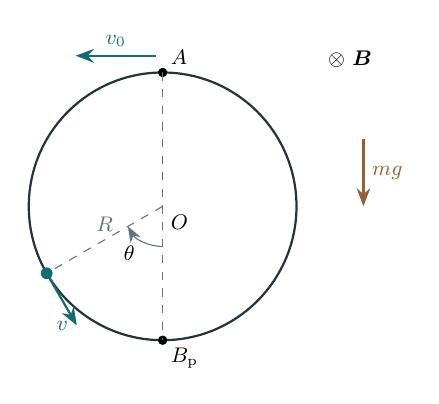
\begin{tikzpicture}[scale=.85,transform shape]

\draw[object] (0,0) circle (2);
\fill (0,2) circle (2pt) node[above right] {$A$};
\fill (0,-2) circle (2pt) node[below right] {$B_{\rm p}$};
\node[below right] at (0,0) {$O$};
\draw[guide] (0,2)--(0,-2);
\draw[motion] (-.1,2.25)--(-1.3,2.25) node[midway,above] {$v_0$};
\draw[guide] (0,0)--(-1.732,-1) node[midway,above] {$R$};
\fill[color=accent] (-1.732,-1) circle (2.5pt);
\draw[motion] (-1.732,-1)--(-1.282,-1.78) node[left] {$v$};
\draw[axis] (0,-.6) arc[start angle=-90,end angle=-150,radius=.6];
\node at (-.5,-.7) {$\theta$};
\draw[force] (3,1)--(3,0) node[midway,right] {$mg$};
\node at (2.8,2.2) {$\otimes\ \boldsymbol B$};

\end{tikzpicture}
\figcaption{图电试2.3\quad 质点沿左半环下降，磁力向心，圆环支持力向外。}
\end{minipage}\end{center}

\par\vspace{5mm}\noindent{\small\color{muted}作答区}\par\vspace{3mm}\noindent\textcolor{rulegray}{\rule{\linewidth}{0.3pt}}\par\vspace{12mm}\noindent\textcolor{rulegray}{\rule{\linewidth}{0.3pt}}

\clearpage

\pdfbookmark[2]{第 4 题 匀强磁场中电阻网络的总安培力}{q4}

\section*{第 4 题\quad 匀强磁场中电阻网络的总安培力}\label{q:4}


平面$\Sigma_1$与$\Sigma_2$相交于直线$MN$，夹角$\phi=45^\circ$。匀强磁场$\boldsymbol B$平行于$\Sigma_1$、垂直$MN$。
$\Sigma_2$内有长方形网络$abcdef$：$a,b$为左下、左上角，$d,e$为右上、右下角，$c,f$分别是上下长边中点。七段$ab,bc,cd,de,ef,fa,fc$均长$l$，且$ab\parallel MN$。各电阻为
\[
R_{ab}=R_{fc}=R_{ed}=R,\quad
R_{af}=R_{bc}=2R,\quad R_{fe}=R_{cd}=4R.
\]
总电流$I$从$a$流入、从$d$流出。求网络所受总磁场力大小，并说明是否需要先求七段电流。
取$\hat e_u$由$a$指向$f$，$\hat e_v$由$a$指向$b$，$\hat n=\hat e_u\times\hat e_v$，选择磁场为
$\boldsymbol B=B(\cos\phi\,\hat e_u+\sin\phi\,\hat n)$。


\begin{center}\begin{minipage}{.98\linewidth}\centering
\begin{tikzpicture}[scale=.7,transform shape]

\coordinate (a) at (0,0);\coordinate (b) at (0,2);
\coordinate (c) at (2,2);\coordinate (d) at (4,2);
\coordinate (e) at (4,0);\coordinate (f) at (2,0);
\foreach \p/\q/\lab in {a/b/R,b/c/2R,c/d/4R,d/e/R,e/f/4R,f/a/2R,f/c/R}{
\draw[object] (\p)--(\q) node[midway,fill=white,inner sep=2pt] {$\lab$};}
\foreach \p in {a,b,c,d,e,f}{\fill (\p) circle (1.6pt);}
\node[below left] at (a) {$a$};\node[above left] at (b) {$b$};
\node[above] at (c) {$c$};\node[above right] at (d) {$d$};
\node[below right] at (e) {$e$};\node[below] at (f) {$f$};
\draw[motion] (-1,0)--(-.15,0) node[midway,above] {$I$};
\draw[motion] (4.15,2)--(5,2) node[midway,above] {$I$};
\draw[axis] (-.7,-.7)--(1,-.7) node[right] {$\hat e_u$};
\draw[axis] (-.7,-.7)--(-.7,1) node[left] {$\hat e_v\parallel MN$};

\begin{scope}[xshift=8cm,yshift=.3cm]
\draw[axis] (0,0)--(2.7,0) node[right] {$\Sigma_2,\hat e_u$};
\draw[axis] (0,0)--(0,2.6) node[above] {$\hat n$};
\draw[motion] (0,0)--(1.8,1.8) node[right] {$\boldsymbol B$};
\draw[guide] (-.5,-.5)--(2.1,2.1) node[above] {$\Sigma_1$};
\draw[axis] (.7,0) arc[start angle=0,end angle=45,radius=.7];
\node at (1,.42) {$\phi$};
\node[align=center] at (1.2,-1) {沿$MN$观察\\截面};
\end{scope}

\end{tikzpicture}
\figcaption{图电试2.4\quad 网络长边为两段l；右侧截面给磁场与网络面的夹角。}
\end{minipage}\end{center}

\par\vspace{5mm}\noindent{\small\color{muted}作答区}\par\vspace{3mm}\noindent\textcolor{rulegray}{\rule{\linewidth}{0.3pt}}\par\vspace{12mm}\noindent\textcolor{rulegray}{\rule{\linewidth}{0.3pt}}

\clearpage

\pdfbookmark[2]{第 5 题 时变磁场中带电弦杆的转动与端点作用力}{q5}

\section*{第 5 题\quad 时变磁场中带电弦杆的转动与端点作用力}\label{q:5}


半径$R$的光滑绝缘圆环固定在水平面内。以环为横截面的竖直圆柱区域内有磁场
$\boldsymbol B=-B(t)\hat z$，其中$B(t)=B_0\sin\omega_0t$、$B_0>0$，$\hat z$竖直向上；柱外磁场为零。采用轴对称的感应电场，忽略附加静电场、自场和辐射。
均匀绝缘刚性细杆$ab$总质量$m$、总正电荷$Q$，其质心$C$距环心$O$为$D=R/2$，两端由光滑的双向径向约束保持在圆周上。电荷分布始终均匀；重力由水平支承平衡，只求水平面内作用力。
$t=0$时杆静止，此后先逆时针转过$2\pi$，再顺时针返回$2\pi$，如此交替。
\begin{enumerate}
\item 求$\omega_0$与$m,Q,B_0$的关系。
\item 求杆在$a,b$端对约束圆环的水平作用力随时间的变化，给出大小和实际方向。
\item 说明上述双向约束若改为只能向杆施加朝向$O$压力的普通单侧内壁，给定运动能否实现。
\end{enumerate}
令$\hat e_r$由$O$指向$C$，$\hat e_t=\hat z\times\hat e_r$；初始杆沿$\hat e_t$，$a$在$C$的负$\hat e_t$侧，$b$在正侧。


\begin{center}\begin{minipage}{.98\linewidth}\centering
\begin{tikzpicture}[scale=.75,transform shape]

\draw[object] (0,0) circle (2);
\draw[object,line width=1.5pt] (1,-1.732)--(1,1.732);
\fill (0,0) circle (1.5pt) node[below left] {$O$};
\fill[color=accent] (1,0) circle (2pt) node[below right] {$C$};
\node[below right] at (1,-1.732) {$a$};
\node[above right] at (1,1.732) {$b$};
\draw[guide] (0,0)--(1,0) node[midway,below] {$D$};
\draw[guide] (0,0)--(1,1.732) node[midway,above left] {$R$};

\draw[axis] (0,0)--(2.7,0) node[right] {$\hat e_r$};
\draw[axis] (1,.15)--(1,2.5) node[above] {$\hat e_t$};
\node at (-1,1) {$\otimes\ B(t)$};
\node at (0,-2.6) {$D=R/2,\quad L=\sqrt3D$};
\node[align=left] at (4.8,1) {杆：均匀$m,Q$\\初始静止\\端点双向径向约束};

\end{tikzpicture}
\figcaption{图电试2.5\quad 俯视水平圆环，a、b的标记随杆运动而保持。}
\end{minipage}\end{center}

\par\vspace{5mm}\noindent{\small\color{muted}作答区}\par\vspace{3mm}\noindent\textcolor{rulegray}{\rule{\linewidth}{0.3pt}}\par\vspace{12mm}\noindent\textcolor{rulegray}{\rule{\linewidth}{0.3pt}}

\end{document}
